\documentclass[10pt, a4paper]{article}
\usepackage[margin=1.5cm]{geometry}
\usepackage{graphicx}

\title{Appunti Tecnologie Open-Source}
\date{A.A. 2020/2021}
\author{Michele Veronesi}

\begin{document}
\maketitle
\tableofcontents

\newpage
\section{Issue Tracking System - ITS}
\textit{Issue}: criticità, evento da gestire\\
\textit{Tracking}: registrare, lasciare traccia
\subsection{Definizione}
Un Issue Tracking System (ITS) è un pacchetto software che gestisce e mantiene una lista di criticità (issue), come richiesto da un'organizzazione.\\
Questo tipo di sistema è spesso usato nei call center di supporto delle aziende per creare, aggiornare e risolvere i problemi segnalati dai clienti o dagli impiegati.\\
In sostanza, è uno strumento che semplifica la gestione del processo di sviluppo e di change management attraverso la gestione di attività diverse (Work item) come: analisi requisiti, sviluppo, test,  bug, release, deploy, change request...\\
Ogni singola "attività minima" (work item) del progetto è gestita mediante un workflow e mantenuta all'interno di un'unica piattaforma e un'unica repository.

\subsection{A cosa serve}
\begin{itemize}
\item Condividere le informazioni tra team di sviluppo, project manager e cliente, infatti offre un unico repository in cui trovare le informazioni e un sistema di notifica.
\item Implementare il processo di misurazione della qualità del progetto
\item Avere un'istantanea dello stato del progetto: attività da fare, in corso d'opera, completate.
\item Decidere cosa rilasciare e quando rilasciare: i work item possono essere assegnati ad una versione
\item Assegnare una priorità alle attività
\item Avere una chiara assegnazione delle responsabilità sulle attività: ogni work item riporta incaricato e assegnatario
\item Tiene la memoria storica di tutti i cambiamenti
\end{itemize}

\subsection{Workflow}
Il workflow è un insieme di stati e transizioni che un work item attraversa durante il suo ciclo di vita. Viene associato ad un progetto e ad uno o più tipi di work item. Permette di registrare tutte le transizioni e i cambi di stato.

\subsection{Collegamenti}
Permettono di mettere in relazione vari work item, anche di differenti tipi (attività, sotto-attività, requisiti, casi di test, ...), sono bidirezionali e vengono registrati come criterio di ricerca. Questo permette di verificare la presenza o meno di relazione tra i work item (per esempio vedere se un requisito è coperto da casi di test).

\subsection{Funzionalità}
\begin{itemize}
\item Ricerca avanzata dei work item
\item Salvataggio di ricerche
\item Esportazione
\item Notifiche
\item Bacheche o board
\item Reporting
\item Dashboard
\item Definizione di Road map e Release Notes
\item Integrazione con il Source code management
\item Integrazione con l’ambiente di sviluppo
\end{itemize}

\subsubsection*{Filtri}
I filtri permettono di ricercare i work item in base ai campi, possono essere salvati per facilitare le ricerche più recenti, i risultati possono essere esportati e \underline{sono la base per creare report, board e dashboard}.

\subsubsection*{Board o bacheche}
Permette di visualizzare i work item di uno o più progetti, offrendo un modo flessibile e interattivo di visualizzazione, gestione e visualizzare dei dati di sintesi sulle attività in corso.\\
È configurata e visualizza i work item ricercati con un filtro.\\
Permette di interagire velocemente con i work items (avanzare di stato, modificare alcuni campi).

\subsection{Configurazione e utilizzo}
\begin{enumerate}
\item Identificare i processi richiesti per la gestione del progetto: vincoli imposti dal cliente, procedure e best practices definiti dai framework di qualità presenti in azienda o imposti dal cliente.
\item Identificare e configurare gli strumenti che permettono di implementare i processi (ITS): identificazione e definizione dei tipi, dei campi custom, dei work flow e dei collegamenti che ci permettono di tracciare le informazioni richieste dal processo.
\end{enumerate}

\begin{itemize}
\item Il manager del ITS: 
	\begin{itemize}
	\item crea un nuovo progetto
	\item definisce il processo da seguire (tipi di work item, campi custom, work flow, collegamenti), seleziona il modello di stima, differenti board e report per processo
	\item Aggiunge gli utenti e assegna ruoli/permessi
	\end{itemize}
	
\item Il manager (capo progetto):
	\begin{itemize}
	\item Definisce le versioni (release)
	\item Definisce le componenti del progetto
	\item Definisce i lavori da svolgere (backlog): priorità, assegnatario e stima
	\item Definisce la prima iterazione
	\item Monitora l’avanzamento e il completamento delle attività (filtri, board, dashboard, report)
	\item Definisce le nuove versioni
	\item Definisce le nuove iterazioni
	\item Definisce, aggiorna e monitora le attività (priorità, verifica stima/consuntivo)
	\item Produce i report richiesti dal cliente (p.es. Calcolo SLA, release log, ...)
	\end{itemize}	 
	
\item Gli utenti (il team di sviluppo):
	\begin{itemize}
	\item Ricevono le notifiche dei work item assegnati
	\item Selezionano i work item in base alle priorità
	\item Avviano e completano la lavorazione: avanzano gli stati del workflow, aggiornano la stima a finire, registrano il tempo impiegato
	\item Completano tutte le attività presenti nell'iterazione
	\item Effettuano il rilascio
	\end{itemize}
\end{itemize}

\subsection{Vantaggi ITS}
\begin{itemize}
\item Implementare un processo e verificarne l’adozione
\item Migliorare e misurare la qualità del progetto
\item Misurare e aumentare la soddisfazione del cliente
\item Migliorare la definizione delle responsabilità
\item Migliorare la comunicazione nel team di sviluppo e con il cliente
\item Aumentare la produttività del team di sviluppo
\item Ridurre le spese e gli sprechi
\end{itemize}
\newpage
\section{Source Code Management - SCM/VCS}
\subsection{Definizione}
I source code management systems (aka version control systems) sono sistemi software che registrano tutte le modifiche avvenute ad un insieme di file. Inoltre permettono la condivisione di file e modifiche, offrendo funzionalità di merging e tracciamento.

\subsection{Vantaggi}
In un team di sviluppo, un SCM permette di:
\begin{itemize}
\item collaborare in modo efficiente sul codice di un prodotto, facilitando l'individuazione e la correzione dei conflitti e la condivisione di commenti e documentazione
\item tracciare ogni modifica (storia del prodotto): fornisce una lista completa dei cambiamenti apportati ad un file, offrendo la possibilità di effettuare un rollback ad una versione precedente
\item lavorare senza interferenze in differenti rami di sviluppo (\textit{branching}); le modifiche avvenute in un branch possono confluire nel master con un merge
\item tracciabilità: tutte le modifiche possono fare riferimento ad un'attività contenuta nel issue tracking system; in ogni istante è possibile capire che attività sono state effettuate in una specifica versione
\end{itemize}

\subsection{Utilizzo}
Con il termine \emph{diff} si indica la differenza tra due versioni di uno stesso file (i.e. cambiamenti tra le righe del file). Un insieme esplicitamente validato di \emph{diff} è detto \emph{commit}. Un \emph{commit} è difatti una nuova versione della codebase, e può esistere localmente o in remoto. L'ultimo \emph{commit} nella history viene chiamato \emph{HEAD}. Questo viene utilizzato per verificare le differenze tra la codebase locale e quella remota. \\
Un \emph{branch} è un puntatore ad un singolo commit. L'\emph{HEAD} fa parte del \emph{master branch}, ogni altro \emph{branch} può integrarsi con il \emph{master} a seguito di un \emph{merge}. \\
L'attività di merging può essere gestita attraverso una \emph{Pull Request}, cioè una procedura di discussione e correzione a seguito della quale una branch può essere integrata con il master. \\
Un \emph{fork} è una copia di una codebase, e permette di lavorare su tale copia liberamente, senza dover richiedere permessi di modifica alla repository originale. Una volta terminate le modifiche è possibile integrarle nella versione originale attraverso una Pull Request.
\subsubsection*{Gitflow}
Il \emph{Gitflow} è un'estensione del pattern \emph{Feature Branch Workflow}. Pensato per progetti di larga scale, il Gitflow prevede la strutturazione dello sviluppo su più branch, assegnando uno specifico ruolo ad ogni branch.
 
\subsection{Tipi di VCS}
\subsubsection*{Locali}
Sono i più vecchi, registrano solo la storia dei cambiamenti utilizzando un \textit{version database} dove viene registrata tutta la storia dei file e salvando sul disco una serie di patch, rappresentanti il cambiamento tra una versione e l'altra. Tuttavia \underline{non gestiscono la condivisione}.

\subsubsection*{Centralizzati}
Più recenti e molto diffusi, aggiungono la condivisone dei file con un version database centralizzato (singolo punto di rottura). Ogni sviluppatore ha solo una versione in locale. Facili da apprendere.

\subsubsection*{Distribuiti}
Simili ai centralizzati, ma il database è distribuito ad ogni noto (anche i client hanno la storia completa dei file). Sono i più diffusi poiché hanno una serie di vantaggi:
\begin{itemize}
\item quando il nodo centrale non è disponibile, è possibile continuare a lavorare localmente registrando i cambiamenti
\item hanno una migliore risoluzione dei conflitti che favorisce la collaborazione
\item permettono di impostare diversi flussi di lavoro (branch)
\end{itemize}
Tuttavia l'apprendimento è più complesso rispetto ai centralizzati.

\section{Il framework Scrum}
\subsection{Definizione}
Scrum è un \textit{processo agile} che nasce per lo sviluppo di progetti complessi (difficili da definire e da risolvere) e che permette di concentrarsi sulla consegna del maggior valore business nel minor tempo possibile.\\
Permette di ispezionare software funzionante rapidamente e ripetutamente (ogni 2-4 settimane).\\
Il business stabilisce le priorità. I team si organizzano per scegliere la strada migliore per consegnare le funzionalità a priorità più alta.\\
Ogni due settimane o un mese, chiunque può vedere il software funzionante e decidere se lasciarlo così o se migliorarlo facendo un altro sprint.

\subsection{Caratteristiche}
\begin{itemize}
\item Leggero
\item Facile da capire
\item Difficile da padroneggiare
\end{itemize}
Si basa su tre pilastri:
\begin{itemize}
\item Trasparenza: linguaggio comune per una conoscenza condivisa, definition of done
\item Controllo: ispezioni pianificate per prevenire variazioni indesiderate
\item Adattamento: aggiustamenti per minimizzare ulteriori deviazioni tramite feedback continuo
\end{itemize}
\begin{minipage}{0.7\textwidth}
	\begin{center}
		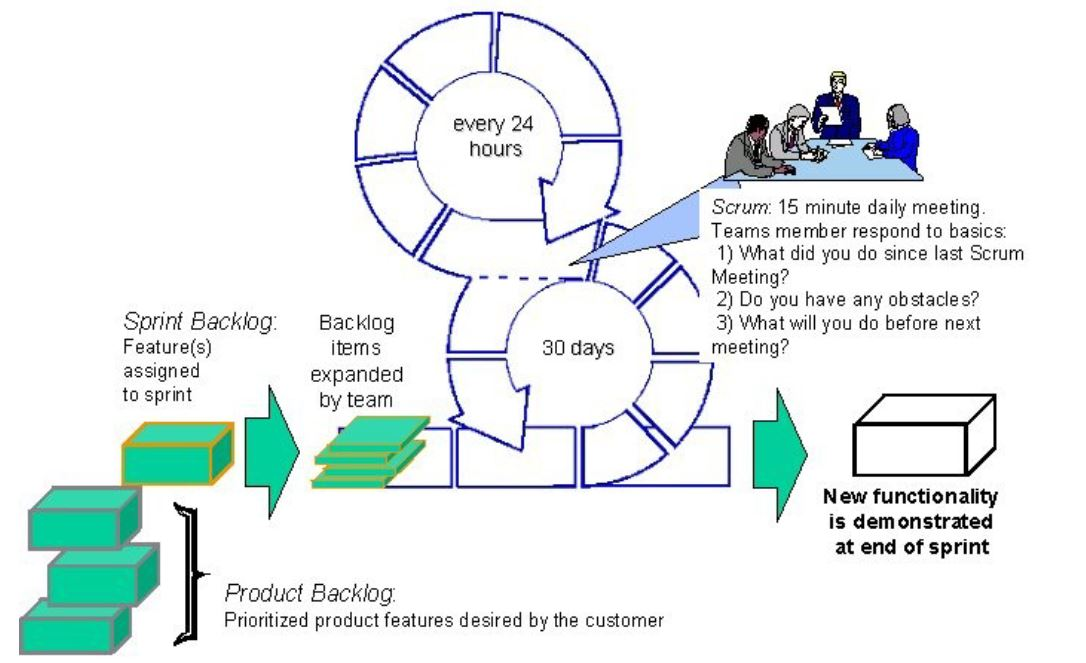
\includegraphics[width=0.95\textwidth]{img/scrum.jpg}
	\end{center}
\end{minipage}
\begin{minipage}{0.3\textwidth}
	Durante lo sprint c'è un daily meeting della durata di 15 minuti in cui si discute l'avanzamento dei lavori locale (ovvero cosa si è fatto ieri e cosa si farà oggi). Inoltre, se qualcuno ha incontrato problemi svolgendo dei work item deve segnalarlo.
\end{minipage}

\begin{itemize}
\item Gruppi che si auto-organizzano
\item Il prodotto evolve attraverso "sprint" mensili (o comunque di durata fissa)
\item I requisiti sono trattati come elementi di una lista detta "product backlog"
\item Non vengono prescritte particolari pratiche ingegneristiche
\item Si basa sull'attività empirica cioè la conoscenza si basa sull'esperienza e  le decisioni si basano su ciò che si è conosciuto
\item Processo iterativo e incrementale per ottimizzare il controllo dello sviluppo e il controllo del rischio
\end{itemize}

\subsubsection*{Sprint}
I progetti Scrum progrediscono attraverso una serie di "sprint", analoghi alle iterazioni della extreme programming (altra pratica agile). Hanno una durata tipica di 2-4 settimane costante, poiché favorisce un ritmo migliore.\\
Durante lo sprint il prodotto viene progettato, realizzato e testato, e durante questo si celebrano tutti gli eventi.\\
\textbf{Non si cambia durante lo sprint:} è necessario che lo scrum master tenga i cambiamenti fuori dallo sprint. Nonostante lo sprint backlog possa essere modificato e rinegoziato tra team di sviluppo e product owner, la durata dello sprint assicura che il rischio di spostarsi da quanto richiesto sia limitato alla durata dello sprint. Uno sprint può essere cancellato se l'obiettivo dello stesso diventa obsoleto, tuttavia ha poco senso vista la durata limitata.

\subsection{Ruoli}
\subsubsection*{Product Owner}
\begin{itemize}
	\item Definisce le caratteristiche del prodotto
	\item Rappresenta il desiderio del committente
	\item Decide date e contenuto del rilascio
	\item È responsabile della redditività del prodotto (ROI)
	\item Definisce le priorità delle caratteristiche del prodotto in base al valore di mercato che gli attribuisce
	\item Adegua le caratteristiche e la priorità ad ogni iterazione, secondo quanto necessario
	\item Responsabile che il Product Backlog sia chiaro e ordinato
	\item Accetta o rifiuta i risultati del lavoro
\end{itemize}

\subsubsection*{Scrum Master}
\begin{itemize}
	\item Rappresenta la conduzione del progetto
	\item Responsabile dell’adozione dei valori e delle pratiche Scrum
	\item Rimuove gli ostacoli 
	\item Si assicura che il gruppo di lavoro sia pienamente operativo e produttivo
	\item Favorisce una stretta cooperazione tra tutti i ruoli e le funzioni
	\item Protegge il gruppo di lavoro da interferenze esterne
	\item Servant leader: aiuta Product Owner e Team di sviluppo condividendo la gestione e le decisioni con il team
\end{itemize}

\subsubsection*{Development Team}
\begin{itemize}
	\item Tipicamente 5-9 persone
	\item Responsabili di realizzare l’incremento in conformità con la Definition of Done
	\item Competenze trasversali (cross functional): programmatori, tester, progettisti di user experience, etc.
	\item Membri di progetto dovrebbero lavorare full-time
	\item Il gruppo di lavoro si auto-organizza: idealmente niente titoli, ma in rari casi può essere una possibilità
\end{itemize}

\subsection{Eventi}
\subsubsection*{Sprint Planning}
Evento time boxed (circa 8 ore per sprint di un mese). L'oggetto di questo è far selezionare dal team di sviluppo gli item da inserire nello sprint backlog, presi dal product backlog. Ciascun task inserito viene quindi stimato (1-16 ore).

\subsubsection*{Daily Scrum}
Detto anche stand up meeting o mischia quotidiana, deve durare al massimo 15 minuti. Non serve a risolvere problemi, ma per sincronizzarsi su quanto fatto e pianificare la giornata per il raggiungimento dello sprint goal. Si aggiorna quindi la scrumboard. Aiuta ad evitare altre riunioni non necessarie.\\
I problemi emersi verranno discussi successivamente con i singoli interessati.\\
\textbf{NB:} non è un SAL (Stato Avanzamento Lavori) per lo scrum master, sono impegni assunti tra pari (team di sviluppo).

\subsubsection*{Sprint Review}
Evento time boxed (circa 4 ore per sprint di un mese).
Il gruppo di lavoro presenta ciò che ha realizzato durante lo sprint tipicamente in forma di demo delle nuove caratteristiche o dell'architettura sottostante (\underline{niente slide,} \underline{max 2 ore per la preparazione}).
Partecipa tutto il gruppo e sono invitati anche gli esterni.

\subsubsection*{Sprint Retrospective}
Evento time boxed (circa 3 ore per sprint di un mese). Si celebra dopo la Sprint Review e prima del prossimo Sprint Planning. Si valuta ciò che sta funzionando e ciò che non sta funzionando:
\begin{itemize}
	\item come migliorare il prodotto?
	\item la Definition of Done è appropriata?
	\item come posso migliorare il prossimo sprint?
\end{itemize}
Vi partecipa tutto il gruppo.
%\newpage
\subsection{Artefatti}
\subsubsection*{Product Backlog}
Raccoglie i requisiti, le funzionalità, i miglioramenti e i fix da realizzare nei prossimi rilasci, essenzialmente una lista di tutti i "desiderata" espressa in modo che sia comprensibile da tutti gli utenti del prodotto o per gli utenti. Le priorità vengono assegnate dal product owner, mentre le stime sono fatte dal development team. Le priorità sono rivalutate all'inizio di ogni sprint, è quindi una lista dinamica che evolve con il prodotto, con un raffinamento continuo.

\subsubsection*{Sprint Backlog}
Ogni componente del Development Team si sceglie qualcosa da fare, il lavoro non è mai assegnato. La stima del lavoro rimanente è aggiornata ogni giorno nel daily scrum, infatti ogni membro del gruppo può modificare parti dello sprint backlog.
Se il lavoro non è chiaro, definire un elemento dello sprint backlog con una stima temporale più ampia, e decomporlo successivamente, aggiornando il lavoro rimanente man mano che diventa più chiaro.

\subsubsection*{Sprint Goal}
Una breve indicazione dell'obiettivo principale dello Sprint. Alcuni esempi:
\begin{itemize}
	\item Database Application: Fare girare l’applicazione anche su SQL Server oltre che su Oracle
	\item Financial Services: Supportare più indicatori tecnici di quanto faccia ABC con dati in tempo reale
\end{itemize}

\subsubsection*{Definition of Done}
Definisce il significato di "svolto" per uno sprint item, ovvero il minimo set di attività per definire che un'attività è completa. Può variare per gruppo di lavoro e dev'essere ben chiara a tutti i membri. È utilizzato per verificare se un'attività è da ritenersi completata.

\subsubsection*{Acceptance Criteria}
Permette di confermare se la storia è completa e funziona come voluto. Sono un insieme di frasi semplici condivise da Product Owner e Development Team. Possono essere incluse con la User Story e rimuovono l’ambiguità dei requisiti.\\
\textit{Esempi}: A user cannot submit a form without completing all the mandatory fields; Information from the form is stored in the registrations database; An acknowledgment email is sent to the user after submitting the form.

\subsubsection*{Sprint burndown chart}
\begin{minipage}{0.6\textwidth}
\begin{center}
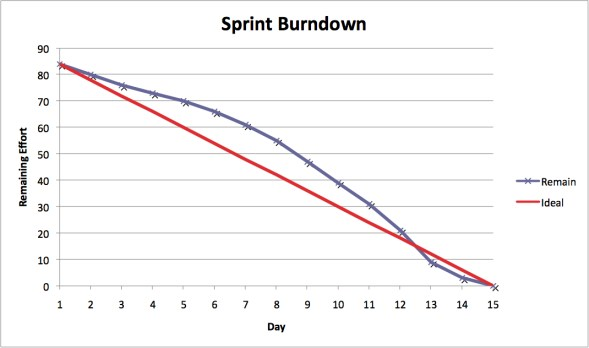
\includegraphics[width=0.95\textwidth]{img/sprint_burndown.jpg}
\end{center}
\end{minipage}
\begin{minipage}{0.4\textwidth}
La linea rossa è la stima, quella blu l'andamento reale. È comune che all'inizio si vada peggio del previsto, tuttavia è facile che poi si vada sotto la stima e si finisca in tempo.
\end{minipage}

\section{Git}
Git è un software di controllo versione distribuito utilizzabile da interfaccia a riga di comando, creato da Linus Torvalds nel 2005.

\subsection{Caratteristiche}
\begin{itemize}
    \item Branching and merging: favorisce lo sviluppo isolato
    \item Piccolo e veloce: la maggior parte delle operazioni viene fatta in locale, solo la condivisione in remoto richiede connessione. È stato realizzato in C per essere leggero e veloce.
    \item Distribuito: ci sono backup multipli della repository creati tramite la \textit{clone}
    \item Integrità: ogni commit è identificato da un ID (checksum SHA-1 di 40-caratteri basato sul contenuto di file o della struttura della directory). Non è possibile cambiare un commit senza modificare l’ID del commit stesso e di i commit successivi.\\
    I commit fanno sempre riferimento al commit padre (il precedente, quello da cui sono cominciate le modifiche).
    \item Staging area: È stata aggiunta un’area di staging dove vengono validati i file modificati che potranno essere versionati con un commit
    \item Free and open source: licenza GNU/GPL 2.0, sorgente gestito su github in repo pubblica.
\end{itemize}
Git salva le variazioni ai file sotto forma di istantanee, non diff. Infatti, ogni volta che si esegue un commit viene fatto uno snapshot dello stato attuale del file system. Inoltre, se un file non subisce modifiche questo sarà un puntatore alla versione precedente, in modo da risparmiare spazio.

\subsection{Aree locali - Stato di un file}
\begin{minipage}{0.4\textwidth}
    In GIT i file della copia locale possono essere:
    \begin{itemize}
        \item Nella \textit{Working directory}, checked out, modificati ma non ancora validati (\textbf{Modified})
        \item Nella \textit{Staging Area}, validati ma non ancora committati. Il commit salva uno snapshot di tutti i file presenti nella staging area (\textbf{Staged})
        \item Nel \textit{Repository locale} (\textbf{Committed})
    \end{itemize}
    Un file appena creato è nello stato di \textbf{Untracked}.
\end{minipage}
\begin{minipage}{0.6\textwidth}
    \begin{center}
        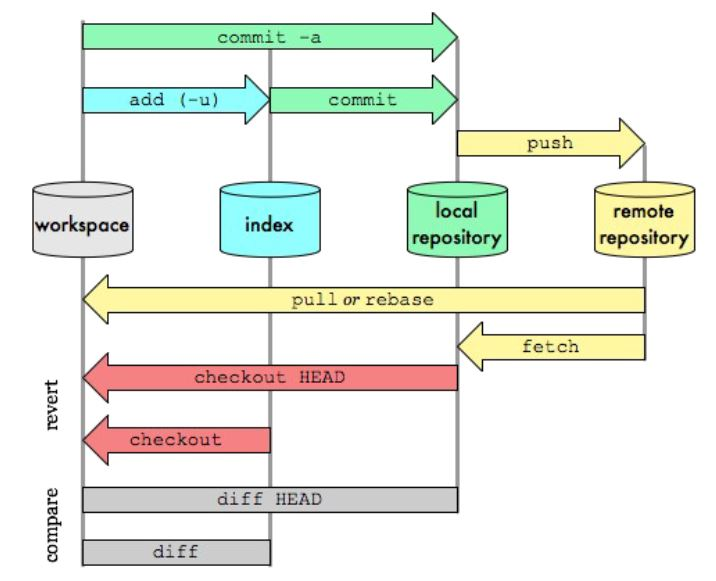
\includegraphics[width=\textwidth]{img/git_command.jpg}
    \end{center}
\end{minipage}

\subsection{Configurazione}
È richiesta una configurazione iniziale dove vengono impostati l’username e l’email da usare per ogni commit:
\begin{itemize}
    \item \verb|git config --global user.name "Bugs Bunny"|
    \item \verb|git config --global user.email bugs@gmail.com|
\end{itemize}
Ci sono tre livelli di visibilità per il config: system (tutti gli utenti), global (utente corrente), local (default, singola repository).
È possibile invocare \verb|git config --list| per avere la lista di tutte le configurazioni.\\\\
Per creare una repository locale si usa \verb|git init| dentro la cartella di un progetto esistente. Tutti i file sono quindi untracked. Viene creata una cartella \verb|.git| contenente la repo.\\
È inoltre possibile clonare una repository remota con \verb|git clone <url>| o locale \verb|git clone <local_directory_path>|.

\subsection{Altri comandi utili}
\begin{itemize}
    \item \verb|git reset HEAD <file_name>|: rimuove un file dalla staging area senza perdere le modifiche
    \item \verb|git checkout -- <file_name>|: rimuove un file dalla staging area perdendo le modifiche
    \item \verb|git status|: vedere lo stato dei file workspace o nella staging area
    \item \verb|git diff|: per vedere cos’è stato modificato ma non ancora validato nella staging area
    \item \verb|git diff --cached|: per vedere cos’è stato modificato nella staging area
    \item \verb|git log|: mostra la lista dei cambiamenti (commit) nel repository locale
    \item \verb|git log -2|: mostra ultimi due commit
    \item \verb|git branch <name>|: crea un nuovo branch indipendente
    \item \verb|git branch|: lista dei branch
    \item \verb|git checkout <branch_name>|: cambia branch su cui si sta lavorando
    \item \verb|git checkout master -> git merge <branch_name>|: effettuare attività di merge di un branch nel master
    \item \verb|git remote|: lista dei repository remoti collegati (possono essere multipli)
    \item \verb|git fetch origin|: recupero i nuovi branch e le modifiche dal remoto senza aggiornare la working copy (senza fare merge)
    \item \verb|git pull origin master|: recupero le ultime modifiche dal repository remoto e aggiorno la working copy (fetch and merge)
    \item \verb|git push origin master|: inviare le modifiche al repository remoto
\end{itemize}

\subsubsection*{Commit keywords}
\begin{itemize}
    \item \verb|git commit -m "close #N"|: questo commit chiude la issue N
    \item \verb|git commit -m "#N message|: aggiunge questo commit alla issue N, con relativo messaggio
\end{itemize}

\subsection{SVN vs GIT}
SVN sta per \textit{subversion}. La principale differenza è che il primo è centralizzato, il secondo distribuito.
Inoltre, in SVN una repository può contenere diversi progetti, questo perché il branching avviene sulle singole cartelle, non nella root. In git questo non è possibile, esiste una repo per ogni progetto.\\
Un'altra importante differenza è che in assenza di connessione, in SVN non è possibile continuare il lavoro di versionamento, visto che il database è singolo e centralizzato.


\section{Build Automation}
\subsection{Definizione}
È il processo di automazione della creazione di build. Ci sono 2 categorie:
\begin{itemize}
    \item \textbf{build-automation utility} (make, gradle, ant...), il cui scopo primario è quello di costruire eseguibili a partire dai diversi file sorgenti che compongono il progetto gestendo attività come compiling e linking
    \item \textbf{build-automation servers} (continuos integration), i quali sono dei server che eseguono utility di build-automation in remoto
\end{itemize}
Il problema iniziale era quello di integrare il codice scritto (è difficile compilare un grande progetto tutto insieme). C'era la necessità di poter scaricare, compilare ed eseguire un progetto open-source per poter collaborare e provare le modifiche apportate.\\\\
Vi sono 2 diversi tipi di build-tools:
\begin{itemize}
    \item \textbf{scripting tools:} tramite l'utilizzo di un linguaggio di scripting si definisce un automatismo (script, make, ant, gradle...)
    \item \textbf{artefact oriented tools:} si basa sulla definizione e creazione di un artefatto (prodotto). Viene configurato il processo di build che è definito nello strumento (Apache Maven, NPM, ...)
\end{itemize}
\subsubsection*{Definizione processo di build}
Il \textit{processo di build} è un insieme di passi che trasformano gli script di build, il codice sorgente, i file di configurazione, la documentazione e i test in un prodotto software distribuibile.

\subsection{Caratteristiche (CRISP)}
\begin{itemize}
    \item \textbf{Completo:} indipendente da fonti non specificate nello script di build. Tutto quello che verrà utilizzato dev'essere specificato.
    \item \textbf{Ripetibile:} accede ai file contenuti nel sistema di gestione del codice sorgente. Un'esecuzione ripetuta dallo stesso risultato. A partire da un commit devo essere in grado di produrre lo stesso artefatto
    \item \textbf{Informativo:} Fornisce informazioni sullo stato del processo (se tutti i passi sono andati a buon fine o meno). Devo accorgermi se ha fallito, come e dove ha fallito
    \item \textbf{Schedulabile:} programmabile ad una certa ora e fatto eseguire automaticamente. I prerequisiti affinché sia schedulabile sono le altre 4 caratteristiche
    \item \textbf{Portabile:} indipendente il più possibile dall'ambiente di esecuzione (eseguibile su un server esterno)
\end{itemize}

\subsection{Apache Maven}
\subsubsection{Definizione}
È uno strumento di gestione di processo basato sul concetto del POM (project - object - model). Può gestire i processi di build, di documentazione, di reportistica a partire dalle informazioni presenti in un file chiamato POM.\\
Viene usato per gestire progetti Java e sfrutta il paradigma \textit{"convention over configuration"}, il quale prevede che ci sia una configurazione minima che vada a descrivere i metadati del nostro progetto, ovvero dove si trovano i sorgenti. La configurazione completa è integrata nello strumento e va bene per la maggior parte dei progetti.\\
Nella configurazione minima specifichiamo solo le caratteristiche del nostro progetto basandoci sul workflow e le configurazioni presenti nello strumento.

\subsubsection{Caratteristiche di Maven}
\begin{itemize}
    \item \textbf{Build Tool:}  sono definite delle Build Lifecycle che permettono di configurare ed eseguire il processo di build (e altri processi). È quindi uno strumento di build e il processo di build è standard.
    \item \textbf{Dependency Management:}  Le dipendenze di progetto vengono specificate nel file di configurazione (pom.xml). Maven si occupa di scaricarle in automatico da dei Repository remoti e salvarle in un repository locale. Tutte le dipendenze vengono identificate da una tripletta detta GAV (group ID - artefact ID - version ID).
    \item \textbf{Remote Repositories:} sono stati definiti dei repository remoti dove sono presenti gran parte delle librerie di progetti opensource e dei plugin utilizzati da maven per implementare e estendere le fasi dei Build Lifecycle. La più famosa è Maven Central, tuttavia possiamo definire le nostre proprietarie.
    \item \textbf{Universal Reuse of Build Logic:}  Le Build Lifecycle, i plugin maven permettono di definire in modo riusabile i principali aspetti richiesti per la gestione di progetto. Tra cui: l’esecuzione del processo di build, l’esecuzione di framework di test (p.es. Junit/TestNG), la creazione di template di progetto (p.es. Applicazioni Java Web o applicazioni costriuite con un determinato framework)
\end{itemize}

\subsubsection{Build Lifecycle}
Maven si basa sul concetto di Build Lifecycle, ovvero il processo per fare build e distribuire un artefatto è ben definito. Questo significa che lo sviluppatore deve imparare un set ristretto di comandi per fare build di qualsiasi progetto Maven, e il file POM assicura che abbiano il risultato desiderato.\\
Ci sono tre build lifecycle già integrati:
\begin{itemize}
    \item \textbf{default lifecycle:} ci permette di andare ad eseguire la compilazione ed esecuzione del nostro pacchetto
    \item \textbf{clean lifecycle:} ci permette di andare a pulire la directory dopo il processo di build
    \item \textbf{site lifecycle:} serve per creare la documentazione del nostro progetto sotto forma di sito web
\end{itemize}
\textbf{Build Lifecyle (default)}\\\\
La default Build Lifecycle è composta dalle seguenti fasi (o goals):
\begin{itemize}
    \item \textit{validate:} controlla che il progetto abbia tutte le informazioni richieste per la fase successiva
    \item \textit{compile:} attraverso i metadati e le dipendenze definite, Maven capisce il compilatore da usare, che dipendenze scaricare, come creare classpath e come compilare il progetto
    \item \textit{test:} recupera le dipendenze di test, crea i classpath ed esegue i test di unità
    \item \textit{package:} parte dai compilati generati precedentemente e crea il pacchetto (es. il file .jar in Java)
    \item \textit{verify:} esegue i test di integrazione sul pacchetto generato
    \item \textit{install:} installa il pacchetto generato nel nostro repository locale in modo da usarlo come dipendenza per altri pacchetti
    \item \textit{deploy:} ci permette di condividere il progetto in un artefact repository e condividere il nostro pacchetto
\end{itemize}
Se un progetto è gestito con maven (ed è presente il file pom.xml) sarà possibile
eseguire il uno dei processi (Build Lifecycle) invocando una delle fasi predefinite.\\
In un qualsiasi progetto gestito con maven, invocando il comando
\verb|mvn install|
verrà effettuata la compilazione, eseguiti i test, costruito l’artefatto e copiato nel
repository locale (eseguite tutte le fasi del Build lifecycle default precedenti a install).
Le fasi vengono gestite da dei plugin maven (attraverso dei \textit{mojo}).

\subsubsection{POM}
Un Project Object Model è l'unità di lavoro fondmanetale di Maven. È in XML e contiene le informazioni in metadati del progetto e le configurazioni desiderate.\\
Quando si esegue un task o un goal, Maven va a vedere le configurazioni nel file POM, se non presenti le va a recuperare nel POM di default di Maven, poi esegue il goal.\\
Le configurazioni che possono essere specificate nel POM sono: le dipendenze del progetto, i plugin o i goal che possono essere eseguiti, i plugin che devono essere usati in determinati goal, dei profili che possono essere attivati ed eseguono determinate operazioni, dei metadati che descrivono la versione del progetto, come identificarlo tra le dipendenze, etc...\\
Tutti i plugin sono mantenuti nell'artefact repository.\\

\subsubsection{Altre utility di Maven}
\textbf{Project Archetypes}\\
Ci permette di andare a definire delle caratteristiche comuni per creare un progetto. Tipicamente se devo cominciare un progetto Java con Maven mi è scomodo ricordare la struttura delle cartelle standard, come creare il POM e come strutturare il progetto.\\
Tramite questa feature, Maven ci mette a disposizione un catalogo di template di progetti da cui possiamo partire.\\\\
\textbf{Mavel plugin e Mojo}\\
Maven in realtà è un orchestratore di plugin Mojo, che vengono attribuiti alle varie fasi del processo di build.\\
I plugin sono dei componenti che vanno a leggere le informazioni presenti nel POM del progetto e hanno la possibilità di andare a fare determinate attività, come compilazione, l'esecuzione dei test, l'analisi statica, la generazione dei javadoc, etc...\\
È molto semplice creare plugin per Maven, grazie all'architettura convention over configuration.\\
I plugin sono a loro volta artefatti Java.

\section{Software Testing}
\subsection{Definizione}
\begin{itemize}
    \item È un'attività di investigazione fatta principalmente per trovare informazioni relative alla qualità del software sotto test. Ha lo scopo di verificare se quello che è stato chiesto dal committente è stato implementato e non contenga errori.
    \item È un processo composto da attività statiche e dinamiche che riguardano la preparazione, la pianificazione e la valutazione delle attività per verificare che un software soddisfi i requisiti e non abbia dei difetti.
\end{itemize}
Il $45\%$ dei difetti è introdotto dal programmatore, il $20\%$ durante l'analisi dei requisiti e il $25\%$ nella progettazione.

\subsection{Categorie di testing}
\begin{itemize}
    \item \textit{Funzionale:} viene condotto per verificare che il prodotto rispetti i requisiti funzionali (richiesti dal committente)
    \item \textit{Non funzionale:} il test fa riferimento a requisiti non funzionali (impliciti, necessari dal problema, non esplicitati dal committente)
    \item \textit{Statico:} non richiedono che il codice venga eseguito, comprendono la revisione dei documenti
    \item \textit{Dinamico:} richiede l'esecuzione del codice o parte di esso
    \item \textit{Verifica:} il prodotto è stato realizzato secondo le specifiche (tecniche) e funziona correttamente. Cercare difetti per migliorare la qualità del software
    \item \textit{Validazione:} il prodotto è stato realizzato rispettando le specifiche dell’utente (requisiti). Convalidare che il software sia conforme ai suoi obiettivi (fit for purpose)
\end{itemize}

\subsection{Processo di test}
Deve essere parallelo al processo di sviluppo, fin dalla definizione dei documenti. Ecco le sue fasi:
\begin{enumerate}
    \item \textit{Test planning:} viene definito il text plan, il documento principale in cui vengono definite le operazioni di test da fare durante il progetto.
    \item \textit{Test control:} sono le azioni correttive e di controllo da attuare nel caso in cui il piano non venga rispettato
    \item \textit{Test analysis:} si decide cosa testare
    \item \textit{Test design:} si decide come effettuare i test
    \item \textit{Test implementation:} si definiscono i casi e gli script di test
    \item \textit{Test execution:} viene effettuata l'attività di test
    \item \textit{Checking result:} si controlla se il test è stato superato/fallito
    \item \textit{Evaluating exit criteria:} si verifica se sono stati raggiunti i requisiti definiti nel text plan
    \item \textit{Test results reporting:} si riporta il progresso rispetto agli exit criteria definiti nel text plan
    \item \textit{Test closure:} chiusura del processo e definizione azioni di miglioramento per i test
\end{enumerate}

\subsection{Sette principi del testing}
\subsubsection*{Il test mostra la presenza di difetti}
Testare un'applicazione può rivelare che uno o più difetti esistono nell'applicazione, ma non può dimostrare che l'applicazione sia priva di errori. È solo possibile progettare casi di test per individuare il maggior numero di errori possibile.

\subsubsection*{Il test esaustivo è impossibile}
A meno che l'applicazione in prova abbia una struttura logica molto semplice e
un input limitato, non è possibile testare tutte le possibili combinazioni di dati e
scenari.\\
Per questo motivo, il rischio e le priorità vengono utilizzati per concentrarsi
sugli aspetti più importanti da testare.\\
Le strategie per selezionare i test sono:
\begin{itemize}
    \item \textit{Risk based testing:} rischio, funzionalità che hanno impatto sul business
    \item \textit{Requirement based:} controllo i requisiti coperti
\end{itemize}

\subsubsection*{Early testing}
Avviare la fase di test il prima possibile permette di risparmiare sui costi del progetto. Prima troviamo il bug e meno ci costa. Il processo di test non deve essere eseguito quando il progetto è al termine, ma deve andare in parallelo con il processo di sviluppo.

\subsubsection*{Defect clustering}
Durante i test, si può osservare che la maggior parte dei difetti segnalati sono
legati a un numero ridotto di moduli all'interno di un sistema.\\
Un piccolo numero di moduli contiene la maggior parte dei difetti nel sistema, circa l'$80\%$ dei problemi si trova nel $20\%$ dei moduli.

\subsubsection*{Paradosso del pesticida}
Se continui a eseguire lo stesso set di test più e più volte (ad ogni nuova
versione), siamo sicuri che non ci saranno più gli stessi difetti scoperti da quei
casi di test.\\
Poiché il sistema si evolve, molti dei difetti precedentemente segnalati vengono
corretti. Ogni volta che viene risolto un errore o è stata aggiunta una nuova
funzionalità, è necessario eseguire tutti i test (di non regressione) per
assicurarsi che il nuovo software modificato non abbia interrotto vecchi errori.\\
Tuttavia, anche questi casi di test di non regressione devono essere modificati
per riflettere le modifiche apportate nel software per essere applicabili.\\
Il set di test va modificato con l'evoluzione del nostro progetto.

\subsubsection*{Il testing dipende dal contesto}
Diverse metodologie, tecniche e tipi di test sono legati al tipo e alla natura
dell'applicazione.\\
Ad esempio, un'applicazione software in un dispositivo medico richiede più test
di un software di giochi.\\
Un software per dispositivi medici richiede test basati sul rischio, essere
conformi con i regolatori dell'industria medica e possibilmente con specifiche
tecniche di progettazione dei test.\\
Un sito web molto popolare, deve superare rigorosi test delle prestazioni e
test di funzionalità per assicurarsi che le prestazioni non siano influenzate dal
carico sui server.

\subsubsection*{Absence of errors fallacy}
Solo perché il test non ha riscontrato alcun difetto nel software, non significa
che il software sia perfetto e pronto per essere rilasciato.
I test eseguiti sono stati davvero progettati per catturare il maggior numero di
difetti? Il software corrispondeva ai requisiti dell'utente?\\
\textbf{Bisogna bilanciare costi, benefici e tempo}.

\subsection{V-model}
\begin{minipage}{0.4\textwidth}
Il processo di test è parallelo a quello di sviluppo, ogni fase dell'attività di sviluppo corrisponde ad una fase di test.
\end{minipage}
\begin{minipage}{0.6\textwidth}
    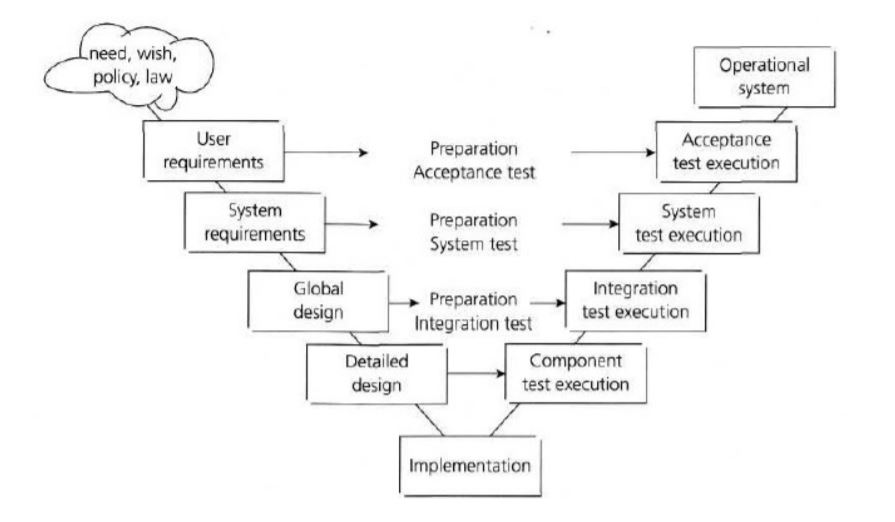
\includegraphics[width=\textwidth]{img/vmodel.jpg}
\end{minipage}

\subsection{Tipi di test}
\subsubsection*{Component testing (unit testing)}
Verificano l’unità: il più piccolo sottosistema possibile (in Java: classe o metodo) che
può essere testato separatamente, sono veloci da eseguire, non dipendono dall'ordine di esecuzione e ogni modifica del codice sorgente dovrebbe scatenare l’esecuzione degli unit test.\\
Il sistema sotto test (SUT) è considerato come \textit{white box}, ovvero possiamo vedere il codice sorgente.

\subsubsection*{Integration test}
Verificano se sono rispettati i contratti di interfaccia tra più moduli o sub-system.\\
I sub-systems possono essere:
\begin{itemize}
    \item Interni: prodotti da noi, già verificati dagli unit test
    \item Esterni: altri componenti con cui integriamo il nostro progetto, es. database, filesystem
\end{itemize}
Questo tipo di test è più lento da configurare e da eseguire. Il SUT è white box.

\subsubsection*{System testing}
Verificano il comportamento dell'intero sistema. Il loro scopo principale è la verifica rispetto alle specifiche tecniche. Il sistema può essere sia white box che black box.\\
Un tipo di system testing sono gli \textbf{smoke test}, il cui obiettivo è quello di trovare gli errori il prima possibile (prima della produzione) o eseguire altri test sul SUT. Verificano le funzionalità del SUT.

\subsubsection*{Acceptance test}
Il sistema è black box e sono eseguiti con il cliente finale. Serve a verificare che i requisiti siano stati implementati correttamente.

\subsubsection*{Non-regression testing}
Verificano che il comportamento del SUT rimanga almeno lo stesso rispetto alla versione precedente (non ci sia un deterioramento qualitativo), si focalizzano su un singolo bug per volta e assicurano che i bug corretti non si presentino ancora.


\section{Unit Testing}
\subsection{Definizione}
In ingegneria del software, per unit testing (testing d'unità o testing unitario) si intende
l'attività di testing (prova, collaudo) di singole unità software. Per unità si intende
normalmente il minimo componente di un programma dotato di funzionamento
autonomo; a seconda del paradigma di programmazione o linguaggio di programmazione,
questo può corrispondere per esempio a una singola funzione nella programmazione
procedurale, o una singola classe o un singolo metodo nella programmazione a oggetti.\\\\
Come le altre forme di testing, lo unit testing può variare da completamente "manuale" ad
automatico. Specialmente nel caso dello unit testing automatico, lo sviluppo dei test case
(cioè delle singole procedure di test) può essere considerato parte integrante dell'attività
di sviluppo (per esempio, nel caso dello sviluppo guidato da test).\\\\
I test di unità sono del codice, prodotto dallo sviluppatore, che esercitano un’unità del
programma.
Per unità si intende una funzionalità atomica che può essere verificata in modo isolato,
in modo da assicurare che il risultato del test non sia influenzato da altre unità.
Nella programmazione ad oggetti un’unità può essere uno o più metodi di una classe, o
un’istanza di una classe. Nella programmazione procedurale un’unità corrisponde ad una
funzione.\\
Vengono sviluppati dal programmatore che sviluppa le unità, per verificare
l’assenza di alcuni errori, e documentare il comportamento dell’unità prodotta.

\subsection{Proprietà desiderabili - A TRIP}
Automatic - Thorough - Repeatable - Independent - Professional

\subsubsection*{Automatic}
I test di unità devono essere eseguiti automaticamente. In ogni progetto deve essere
disponibile un “automazione a comando” che permetta a tutti di invocare e far eseguire tutti
o una parte dei test di unità in modo semplice.\\
Durante la fase di sviluppo del progetto è importante che i test possano eseguire:
\begin{itemize}
\item \textit{In modo rapido:} I test di unità devono essere semplici e la loro esecuzione non deve
impiegare più di pochi secondi.
\item \textit{Senza richiedere l’interazione umana:} Se un test di unità richiede che alcuni parametri
siano inseriti, ogni volta, manualmente da uno sviluppatore, questo non permetterebbe
di eseguire tutti i test del progetto in modo automatico a determinate ore del giorno.
\item \textit{In modo autonomo:} L’automazione che effettua l’esecuzione dei test di unità deve essere in grado di capire quando e dove i test falliscono ed avvisare gli sviluppatori. In
questo modo gli sviluppatori saranno interrotti, dall’attività lavorativa, solo quando uno o più test falliranno. Serve un metodo per far fallire la build se il test fallisce.
\end{itemize}

\subsubsection*{Thorough (esaustivi)}
Dei buoni test di unità devono essere esaustivi e accurati, devono verificare il
comportamento di qualsiasi parte del progetto che potrebbe creare degli errori.\\
Esistono degli strumenti che permettono di misurare se ogni parte del progetto è stata eseguita durante la fase di test, e possono calcolare:
\begin{itemize}
\item La percentuale di righe di codice che vengono esercitate attraverso i test di unità nel progetto
\item La percentuale di possibili diramazioni che vengono eseguiti dai test di unità
\item Il numero di eccezioni che vengono controllate attraverso i test
\item Altri dati che permettono di capire dove il progetto è carente di test di unità
\end{itemize}
Come si può intuire, non è detto che se in un progetto viene eseguito il 100\% del codice dai test di unità questo è privo di errori.

\subsubsection*{Repeatable (ripetibili)}
I test di unità devono produrre sempre lo stesso risultato con lo stesso input. I test non devono seguire un ordine.\\
Per essere ripetibili, i test di unità devono avere l seguenti caratteristiche:
\begin{itemize}
\item \textit{Essere indipendenti dall’ordine di esecuzione:} L’ordine di esecuzione dei test di
unità non deve influenzare il risultato. Per questo è necessario che i test siano
indipendenti l'uno dall'altro. Un test non può essere precondizione di un altro.
\item \textit{Essere indipendenti dall’ambiente di esecuzione:} L’esecuzione dei test non deve dipendere da risorse esterne al progetto o da risorse non gestite nel VCS. Se alcune unità devono utilizzare risorse esterne (p.es. database) è consigliato utilizzare la tecnica Mock Object per simulare il comportamento di queste componenti (oggetti finti che simulano il comportamento dei subsystem esterni, classe di simulazione). Esistono dei framework specifici per questo tipo di oggetti.
\end{itemize}

\subsubsection*{Independent (indipendenti)}
I test di unità devono essere il più possibile indipendenti dall'ambiente di esecuzione,
dagli elementi esterni al progetto e dall'ordine di esecuzione. Quando si scrive un
test è consigliato verificare il comportamento di un singolo aspetto del progetto (in
questo modo si riesce ad identificare univocamente un'errore). Questo non significa che
un test di un'unità deve avere solo una asserzione, ma deve controllare solo un metodo
o più metodi che realizzano un aspetto di una funzionalità del progetto.\\
Se il test è indipendente il suo comportamento sarà ripetibile nel tempo, perché il suo
comportamento non dipenderà dalle altre unità del progetto. La ripetibilità del test è un
aspetto che permette di capire se il test è indipendente.

\subsubsection*{Professional}
Poiché i test di unità sono codice, devono essere scritti e mantenuti con la stessa
professionalità del codice di produzione del progetto.\\
Visto che i buoni test di unità devono essere esaustivi, è ragionevole che il numero di
linee di codice per realizzare i test sia pari o a volte superiore delle linee di codice in
produzione.

\subsection{Framework per unit testing}
Per creare i test di unità sono necessari i seguenti componenti:
\begin{itemize}
\item Un modo per configurare l’ambiente di esecuzione del test
\item Un modo per selezionare un test o un insieme di test da eseguire
\item Un modo per analizzare i valori aspettati, prodotti dalle unità
\item Un modo standard per eseguire ed esprimere se il test è stato superato, se è fallito o
se sono stati prodotti degli errori
\end{itemize}
Nel corso si vedrà JUnit 4, il quale ha tutte le caratteristiche elencate.
% TODO: integrare con link delle slide

\subsection{Come verificare i risultati}
Verificare se i risultati che essa produce sono corretti.
Per corretto si intende che il risultato atteso sia uguale al risultato prodotto dall’unità.
Capita che i requisiti non sono chiari, o possono cambiare nel tempo. In questi casi i test
di unità sono un buon punto di partenza per documentare nel codice, come uno
sviluppatore ha interpretato i requisiti e descrivere il comportamento delle unità
realizzate.\\
I test di unità descrivono come le unità che abbiamo prodotto dovrebbero funzionare.

\subsubsection*{Boundary conditions (CORRECT)}
\begin{itemize}
\item Conformance - I valori sono conformi al formato atteso? [ A+1 ] [1-2]
\item Ordering - I valori seguono o non seguono un ordine? [++ 1 2 3 ]
\item Range - I valori sono all’interno di un valore di minimo e massimo appropriato?
[2147483647 + 2]
\item Reference - I valori possono provenire da codice che si riferisce a dati esterni che non
sono sotto il controllo del codice?
\item Existence - I valori esistono (non sono nulli, non sono zero, sono presenti in un
determinato insieme)? [null]
\item Cardinality - I valori sono nella quantità desiderata? [1 + 2 + 3 + ]
\item Time - I valori rispettano un ordine temporale?
\end{itemize}
Con il termine valore si fa riferimento sia ai parametri di input dei metodi di un'unità, che ai dati interni all'unità e ai risultati che questa produce.

\subsubsection*{Check inverse relationship}
Alcune unità possono o devono essere verificati tramite l'applicazione della loro
funzionalità inversa.\\
Esempi:
\begin{itemize}
\item Calcolare la radice quadrata di un numero. Per testare se la radice quadrata è corretta è
possibile elevare al quadrato il risultato ritornato dall'unità e confrontarlo con il dato di
partenza.
\item Inserimento di un un elemento in una pila. Il modo più semplice per verificare se
l'inserimento è andato a buon fine è quello di effettuare un prelevamento dalla pila e
controllare che l'elemento ritornato sia l'elemento di partenza.
\end{itemize}

\subsubsection*{Cross-check Using Other Means}
Utilizzare uno strumento esistente (oracolo) per verificare se la nuova unità ha lo stesso
comportamento.\\
Esempio: migrazione da un vecchio sistema ad uno nuovo appena realizzato,
si utilizza il vecchio sistema per verificare che quello nuovo abbia lo stesso
comportamento.

\subsubsection*{Force error contitions}
Nel mondo reale gli errori accadono. Una buona norma, per creare un buon progetto, è
quello di ricreare le condizioni di errore e verificare che il progetto funzioni come ci si
aspetta in queste condizioni.

\subsubsection*{Performance caratteristics}
I test di unità devono essere veloci perché devono poter essere eseguiti molto spesso, sia nelle workstation degli sviluppatori che negli automation server.

\subsection{Test driven development}
Il test-driven development (abbreviato in TDD), è un modello di sviluppo del software che prevede
che la stesura dei test automatici avvenga prima di quella del software che deve essere sottoposto
a test, e che lo sviluppo del software applicativo sia orientato esclusivamente all'obiettivo di
passare i test automatici precedentemente predisposti.
Più in dettaglio, il TDD prevede la ripetizione di un breve ciclo di sviluppo in tre fasi, detto "ciclo TDD":
\begin{enumerate}
\item Nella prima fase (detta "fase rossa"), il programmatore scrive un test automatico per la nuova
funzione da sviluppare, che deve fallire in quanto la funzione non è stata ancora realizzata.
\item Nella seconda fase (detta "fase verde"), il programmatore sviluppa la quantità minima di codice
necessaria per passare il test.
\item Nella terza fase (detta "fase grigia" o di refactoring), il programmatore esegue il refactoring del codice per adeguarlo a determinati standard di qualità.
\end{enumerate}




















\end{document}